\chapter{Experimentação}
\label{cap:estudo_de_caso}

Este trabalho descreve a realização de um experimento que visa evidenciar a operacionalidade do SIAPE e sua aderência à \iQuatroZero. Além disso, mostra algumas comparações com o protótipo chamado Produto UFAM, o qual sintetiza o sistema flexível \iTresZero.

Primeiramente descreve-se as características e funcionamento do produto UFAM. Por fim, são descritos o cenário e a configuração do SIAPE e a experimentação é realizada. Os resultados são então registrados para uma posterior comparação (Capítulo 5) com o Produto UFAM.

%============================PRODUTO UFAM===============================================


\section{Produto UFAM}	

\subsection{Descrição do Produto UFAM}

O Produto UFAM é um sistema de carimbos de letras para a montagem de anagramas a partir de um CLP e módulos pneumáticos, tal como os sistemas de montagem atuais, isto é, \iTresZero.

O Produto UFAM originou a parte de hardware do SIAPE com as devidas melhorias e restrições impostas pelo cliente. Então, as características do SIAPE são herdadas tanto de ambientes \iTresZero, quanto de ambientes \iQuatroZero.
	 
O Produto UFAM é o resultado da integração entre seis subsistemas: um sistema microcontrolado, que utiliza entradas analógicas e digitais como entradas e saídas do sistema; um sistema de atuadores, composto por um motor DC alimentado com 24V DC, lâmpadas de 24V DC, uma lâmpada de 127V AC, e eletroválvulas de 6bar que são controladas por solenóides de 24V DC; um sistema de sensores composto por 6 sensores magnéticos e 1 sensor de presença; um sistema de ar comprimido com cinco ramificações de 6 bar. Esses sistemas são alimentados com por uma fonte elétrica que fornece 127V DC e 24V DC e tem a sua inicialização dada por um operador humano que liga o sistema e insere um palete para que seja processado pelo sistema de manufatura. A Figura \ref{F130} mostra o Produto UFAM.
	 
	 
\begin{figure}
	\centering
	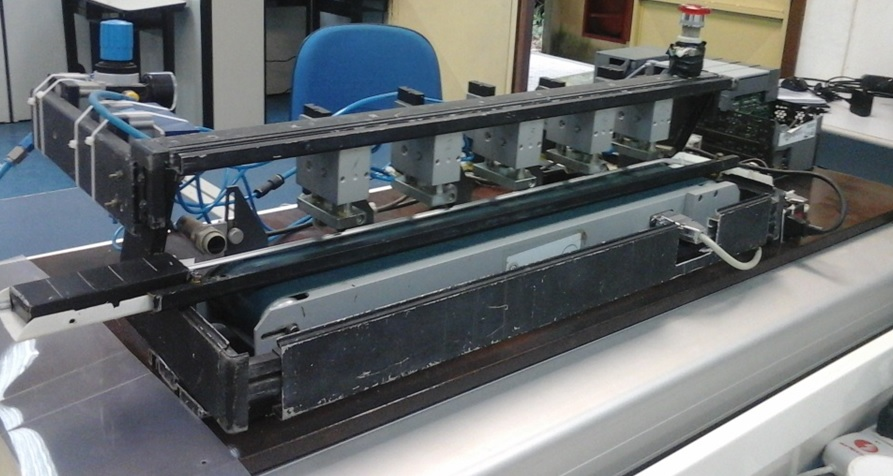
\includegraphics[width=12cm, height=6cm]{F130_PRODUTO_UFAM.jpg} 
	\caption{Produto UFAM}
	\label{F130}
\end{figure}
	 
	 
\subsubsection{Descrição de funcionamento do Produto UFAM}

A Figura~\ref{F131} ilustra o Diagrama em bloco do Produto UFAM e a Tabela~\ref{T15} identifica a legenda dos componentes constantes no diagrama neste diagrama em blocos.

\begin{figure}
 	\centering
 	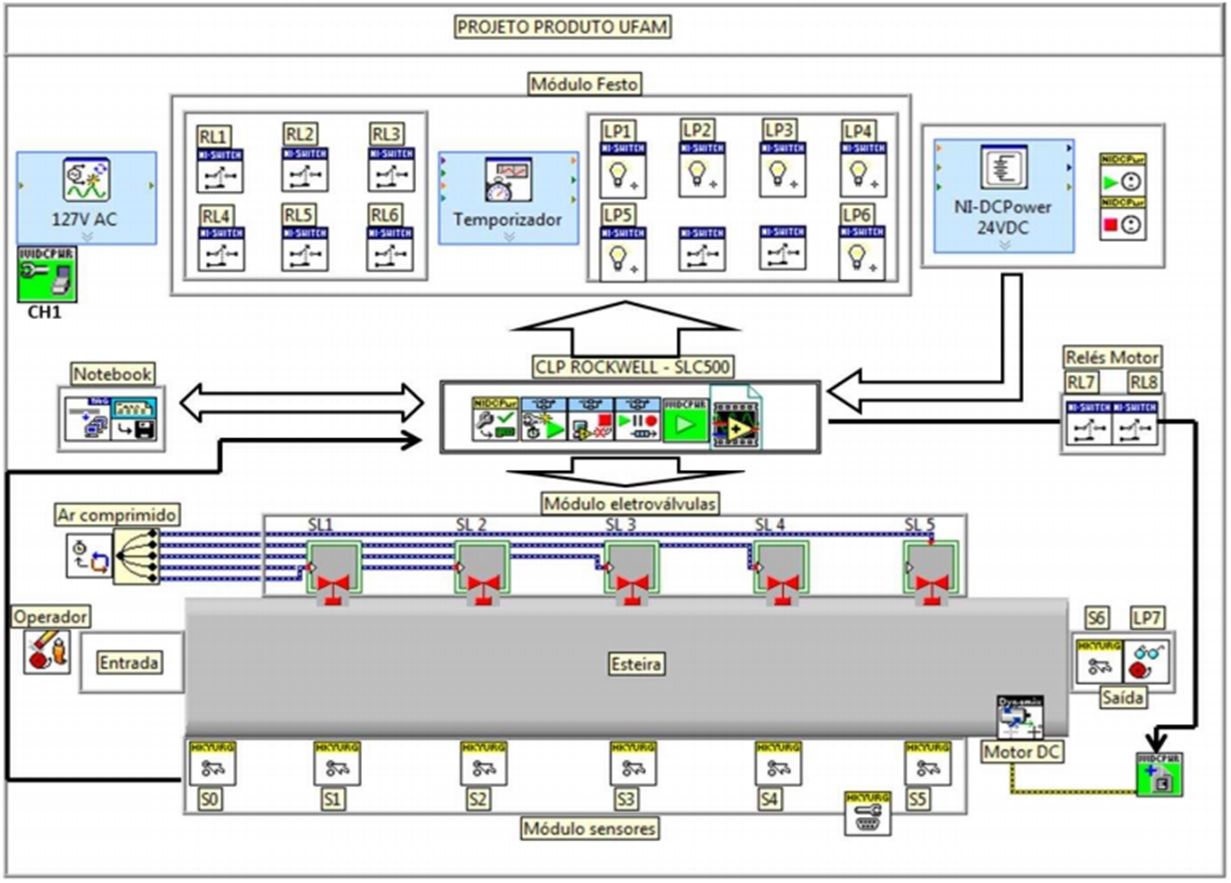
\includegraphics[width=16cm, height=12cm]{F131_PRODUTO_UFAM_ARQUITETURA.jpg} 
 	\caption{Diagrama em bloco do Produto UFAM}
 	\label{F131}
\end{figure}   	
 
Para que o sistema seja energizado o operador necessita acionar a chave 1 (CH1: on-off) para a alimentação da rede 127/220VAC ser aplicada ao sistema elétrico do hardware do Produto UFAM. O código Ladder do Produto UFAM está configurado para realizar a energização sequencial das eletroválvulas no tempo de 0,5 segundos entre as mesmas. Assim sendo, tem-se como resultado o posicionamento das eletroválvulas iniciando por SL1 e finalizado por SL5. O palete, ao ser detectado pelo sensor 0 (S0) aciona o motor DC que movimenta a esteira conduzindo o bloco na direção do sensor 1 (S1). 
	 
\begin{table}
 	\centering
 	\caption{Legenda da planta do produto UFAM}
 	\begin{tabular}{ |c | p{2cm}| p{9cm} | } \hline
 		\textbf{ Item} 	   & \textbf{Tipo}	&\textbf{Descrição}  \\ \hline
 		
 		1 & LP1 a LP5 & Lâmpada correspondente ao solenóide SL1 a SL5 \\ \hline
 		2 &LP6 & Lâmpada correspondente ao sensor 0 \\ \hline
 		3 &LP7 & Lâmpada correspondente ao sensor 6 \\ \hline
 		4 &RL1 a RL6 & Relé correspondente aos sensores S0 a S5 \\ \hline
 		5 &RL7 & Relé do motor DC  \\ \hline
 		6 &RL8 & Relé do motor DC  \\ \hline
 		7 &S0 & Sensor de Entrada \\ \hline
 		8 &S1 & Sensor correspondente à letra M \\ \hline
 		9 &S2 & Sensor correspondente à letra A \\ \hline
 		10 &S3 & Sensor correspondente à letra F \\ \hline
 		11 &S4 & Sensor correspondente à letra T \\ \hline
 		12 &S5 & Sensor correspondente à letra U \\ \hline
 		13 &S6 & Sensor de Saída \\ \hline
 		14 &SL1 & Solenóide correspondente à letra M \\ \hline
 		15 &SL2 & Solenóide correspondente à letra A \\ \hline
 		16 &SL3 & Solenóide correspondente à letra F \\ \hline
 		17 &SL4 & Solenóide correspondente à letra T \\ \hline
 		18 &SL5 & Solenóide correspondente à letra U \\ \hline
 		19 & CH1& Chave on-off \\ \hline				 	   			
 	\end{tabular}												
 	\label{T15}\par
 	%	Fonte: Hiram Amaral
\end{table}
 
A lâmpada LP6 identifica o status do sensor 0 (S0). O palete, ao ser detectado por S1, interrompe a alimentação do motor DC. Neste momento, a alimentação da eletroválvula correspondente a S1 é interrompida e o ar comprimido na eletroválvula, pressiona-a sobre o palete estampando a letra M. Após a estampagem, a alimentação da eletroválvula e do motor retorna, movendo a eletroválvula para a posição inicial e movimenta a esteira para frente.

O palete, agora com a letra M estampada, move-se em direção aos demais sensores que repete a ação de estampagem para as demais letras até completar a palavra do UFAM. Ao chegar no fim da esteira, o bloco estampado é captado por S6 que interrompe a alimentação do sistema e aciona o sinalizador (LP7) para que o operador retire o produto UFAM da esteira e insira um novo palete. O processo então reinicia até que a produção seja atingida. 	  
	 



%========================================================================================

\section{Experimentação - Configurações do SIAPE}

%Um ambiente de produção deve ser montado e configurado para a realização das atividades a serem realizadas na experimentação. O estudo de caso deve ser descrito, o ambiente de produção configurado para que se inicie as atividades. 

Esta seção trata da descrição de um experimento com o SIAPE e suas configurações para produção.

\subsection{Objetivos da configuração para a experimentação}

Dentre os principais objetivos da configuração para a experimentação pode-se se destacar os seguintes:

\begin{description}
\item [1]possibilitar que todos os dispositivos especificados estejam  funcionando em  rede;
\item [2]conseguir fazer com os equipamentos estejam interligados para alimentar os circuitos quando necessário;
\item [3]monitorar as operações de uma forma que o software possa funcionar com o tempo correto;
\item [4]possibilitar as realizações das habilidades dos agentes  nas operações necessárias à realização do plano.
\end{description}

\subsection{A configuração para a experimentação}

A Figura \ref{F103} ilustra uma visão simplificada  do estudo de caso que será evoluída até que a configuração do sistema seja atingida.

	\begin{figure}[h]
		\centering
		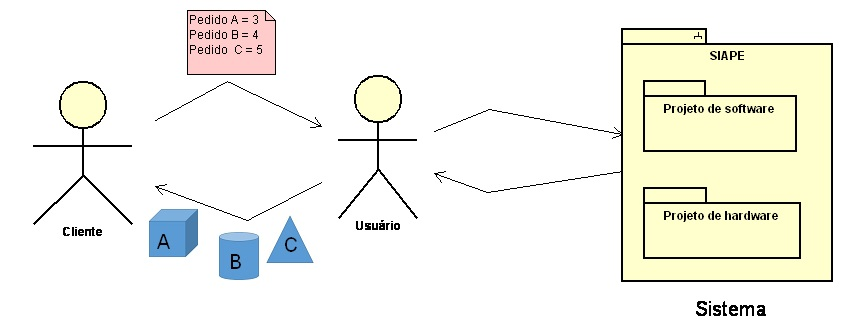
\includegraphics[width=16cm, height=6cm]{F103_SIAPE_ESTUDO_DE_CASO.jpg} 
		\caption{SIAPE - Experimentação}
		\label{F103}
	\end{figure}

O estudo de caso é composto por uma solicitação de um cliente. Essa solicitação é composta por três pedidos de produção conforme segue:

\begin{description}
	\item[Pedido 1 -] Produto A: A  palavra UFAM; Quantidade = 03 unidades
	\item[Pedido 2 -] Produto  B: A  palavra UTAM; Quantidade = 04 unidades
	\item[Pedido 3 -] Produto  C: A palavra UEA; Quantidade = 05 unidades
\end{description} 

A Realização da  solicitação é processada seguindo os passos a seguir:

\begin{enumerate}
	\item O Cliente solicita os pedidos de produção ao operador.
	\item O Operador insere os pedidos no sistema.
	\item O Sistema realiza os pedidos e retorna os produtos para o operador.
	\item O Operador finalmente atende à solicitação do cliente e entrega os produtos solicitados ao cliente.
\end{enumerate} 

\subsection{Descrições de software e hardware do ambiente de produção.}


O cenário é desenvolvido no ambiente denominado de Ambiente de Produção. A Figura~\ref{F104} ilustra os componentes básicos do sistema e suas descrições de hardware e de software são feitas nas tabelas a seguir.

	\begin{figure}
		\centering
		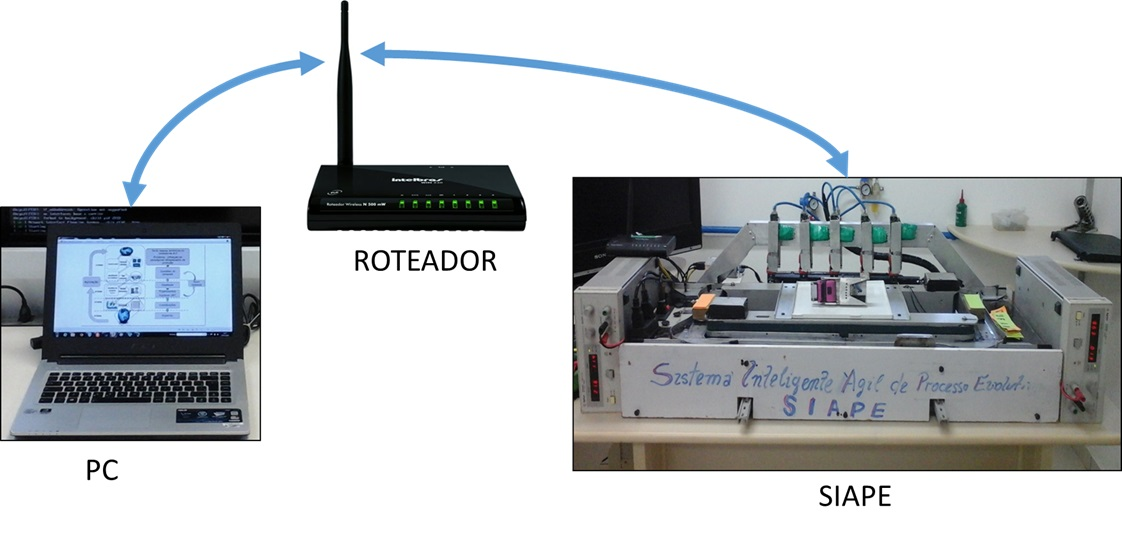
\includegraphics[width=16cm, height=8cm]{F104_SIAPE_AMBIENTE.jpg} 
		\caption{Ambiente de produção para o estudo de caso}
		\label{F104}
	\end{figure}

	
	O PC deve estar preparado com as características de hardware e software descritas nas Tabelas~\ref{T2} e~\ref{T3} para se conectar à rede existente no roteador:
	
	\begin{table}
		\centering
		\caption{PC - Itens características de software}
		\begin{tabular}{|p{4cm}| p{11cm}| c| } \hline
			\textbf{ Item }	   & \textbf{ Descrição}	 \\ \hline
			\textbf{1. Java}   & Linguagem Java instalada e configurada \\ \hline
			\textbf{2. IDE}    & O Interface do Ambiente de 
			Desenvolvimento dor NetBeans instalada e configurada \\ \hline
			\textbf{3. Jade}		  & Framework Jade feito em Java\\ \hline
			\textbf{4. Raspberry pi}	 & Placa Raspberry Pi configurada interface  elétrica\\ \hline
			\textbf{5. pi4j}	 & Biblioteca para trabalhar com as entradas
			 e saídas de comunicação com sensores e atuadores\\ \hline
			\textbf{6. Swing}	 & Biblioteca para interface feita em Java\\ \hline
			\textbf{7. EPSCore}	 & Biblioteca desenvolvida para a aplicação no SIAPE\\ \hline
			\textbf{8. MainSiape}	 & Código para criar plataforma Jade e o agente YPA\\ \hline
			\textbf{9. AcHw}	 & Código para criar o agente Acesso Hardware\\ \hline
			\textbf{10. Order}	 & Código para criar o agente Order\\ \hline
		\end{tabular}
		\label{T2}
		%	Fonte: Hiram Amaral
	\end{table}
	
	\begin{table}
		\centering
		\caption{PC - Itens características de hardware}
		\begin{tabular}{|p{4cm}| p{11cm}| l|} \hline
			\textbf{ Item }	   & \textbf{ Descrição}	 \\ \hline
			\textbf{1. Arquitetura }   & AMD 64 bits \\ \hline
			\textbf{2. Processadores}       & 4 Processadores Lógicos \\ \hline
			\textbf{3. Sist. Operac}	& Windows e Linux\\ \hline
			\textbf{4. Processador}	   &  Intel(R) Core(TM) i7-4510U CPU @ 2.00GHz, 2001 Mhz, 2 Núcleo(s)\\ \hline
			\textbf{5. Memória}	         & Memória Física (RAM) Instalada	8,00 GB\\ \hline
		\end{tabular}
		\label{T3}\par
		%	Fonte: Hiram Amaral
	\end{table}
	
O roteador deve ter as características de hardware e software descritas nas Tabelas \ref{T4} e \ref{T5}:
		
	\begin{table}
		\centering
		\caption{Roteador - Itens características  de software}
		\begin{tabular}{|p{4cm}| p{11cm}| l } \hline
			\textbf{ Item }	   & \textbf{ Descrição}	 \\ \hline
			\textbf{1. Rede }   & MeDSE siape 2\\ \hline
			\textbf{2. IP}    & 10.0.0.1\\ \hline
			\textbf{3. Interface }		  & 150 Mbps operando dentro dos padrões IEEE802.11b/g/n\\ \hline
			\textbf{4. Processador}	 &  Intel(R) Core(TM) i7-4510U CPU @ 2.00GHz, 2001Mhz, 2 Núcleo(s)\\ \hline
			\textbf{5. Modo repetidor}	 & DHCP cliente e servidor\\ \hline
		\end{tabular}
		\label{T4}\par
		%	Fonte: Hiram Amaral
	\end{table}	
	
	
			\begin{table}
				\centering
				\caption{Roteador - Itens características  de hardware}
				\begin{tabular}{|p{4cm}| p{11cm}|l| } \hline
			\textbf{ Item }	   & \textbf{ Descrição}	 \\ \hline
					\textbf{1. Chipset }   & Realtek RTL8196C\\ \hline
					\textbf{2. Memória Flash}    & 2 MB\\ \hline
					\textbf{3. Antena }		  & 5 dBi\\ \hline				
					\textbf{4. Potência}	 &  700mW (27dBm) via hardware\\ \hline
					\textbf{5. Modo repetidor}	 & DHCP cliente e servidor\\ \hline
					\textbf{6. Portas}	 & 01 porta WAN RJ45 e 04 portas LAN RJ45\\ \hline
				\end{tabular}
				\label{T5}\par
				%	Fonte: Hiram Amaral
			\end{table}		


O SIAPE deve ter as características de hardware descritas na Tabela \ref{T6}:

\begin{table}
	\centering
	\caption{SIAPE - Itens características  de hardware}
	\begin{tabular}{|p{4cm}| p{11cm}|l| } \hline
			\textbf{ Item }	   & \textbf{ Descrição}	 \\ \hline
		\textbf{1. M }   & Módulo mecânico\\ \hline
		\textbf{2. E}    & Módulo eletrônico\\ \hline
		\textbf{3.  EEm}  & Entidade eletro-mecânica das letras\\ \hline				
		\textbf{5. EEe}	 & Entidade eletro-mecânica da esteira\\ \hline
	\end{tabular}
	\label{T6}\par
	%	Fonte: Hiram Amaral
\end{table}	


\subsection{Configuração do ambiente de produção.}
Para que o cenário seja realizado no ambiente de produção, este deve ser configurado seguindo os procedimentos relacionados de 1 a 6 que são descritos a seguir e devem ser acompanhados pela ilustração da Figura \ref{F105}.\par 
		\begin{figure}[!h]
			\centering
			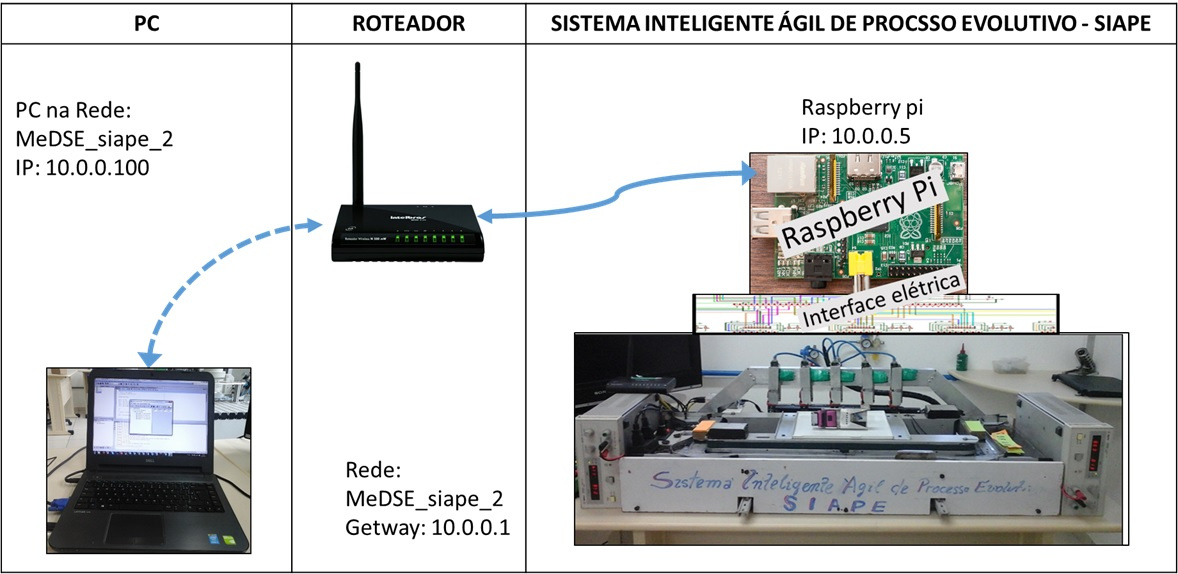
\includegraphics[width=16cm, height=7cm]{F105_SIAPE_ESTUDOD_DE_CASO1.jpg} 
			\caption{Configuração do Ambiente de produção para a experimentação}
			\label{F105}
		\end{figure}
		
		
%		\begin{description}
	\textbf{1.} Ligar o sistema -
			Ao ligar a chave \textit{power} do sistema os dispositivos PC, Roteador e SIAPE são energizados e estarão preparados para serem configurados. 
			
	\begin{figure}[!h]
		\centering
		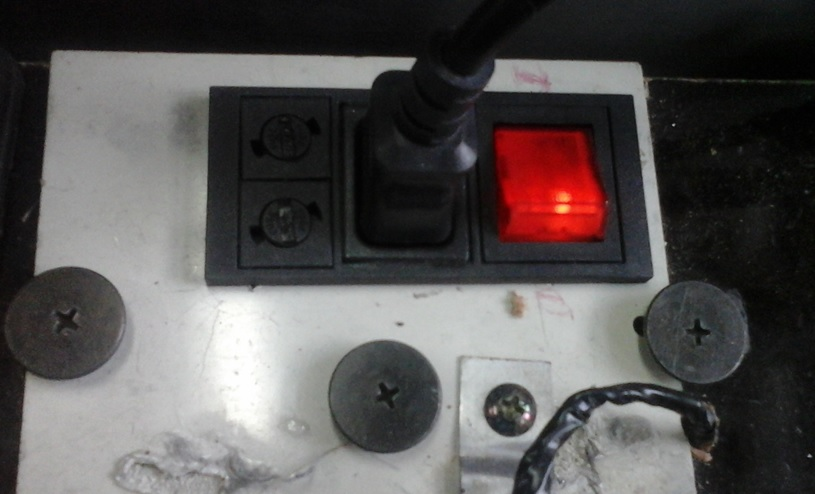
\includegraphics[width=10cm, height=5cm]{F106_SIAPE_POWER.jpg} 
		\caption{Power dos dispositivos}
		\label{F106}
	\end{figure}	
			
			
		\textbf{2.} Configurar o roteador -
			Uma rede é estabelecida no roteador com o nome de MeDSE siape com o IP:10.0.0.1. Esta rede será acessada pelo Raspberry Pi e pelos agentes via Protocolos FIPA que são codificados em Java. 
			
				\begin{figure}[!h]
					\centering
					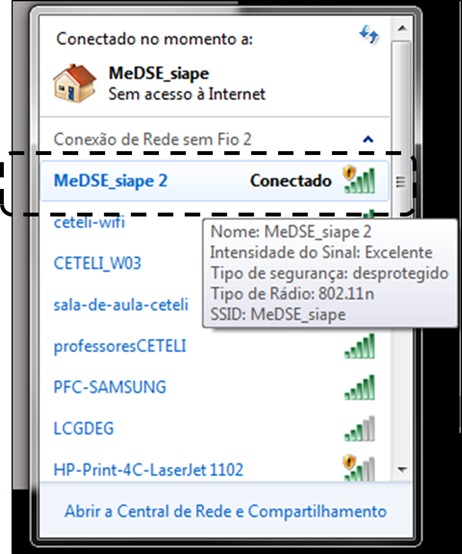
\includegraphics[width=10cm, height=5cm]{F107_SIAPE_MeDSE_siape.jpg} 
					\caption{Rede MeDSE siape - ip:10.0.0.1}
					\label{F107}
				\end{figure}
			
		\textbf{3.} Configurar o Raspberry Pi -
			O Raspberry Pi é configurado com um IP fixo de número 10.0.0.5 e acessa a Rede MeDSE siape via cabo RJ45. O Raspberry é conectado diretamente à interface elétrica e fornecerá ao agente YPA a informação dos módulos presentes na interface  elétrica;
			
			
				\begin{figure}[!h]
					\centering
					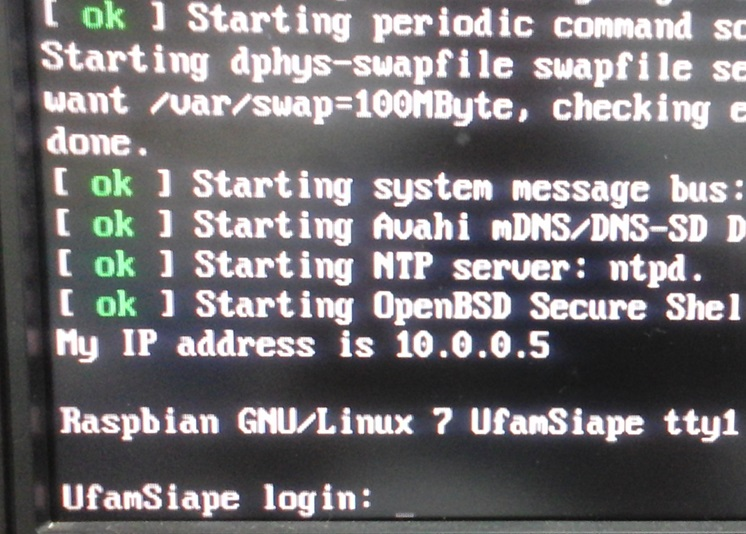
\includegraphics[width=10cm, height=4cm]{F108_SIAPE_RPI.jpg} 
					\caption{Rede MeDSE siape - Raspberry Pi - 10.0.0.5}
					\label{F108}
				\end{figure}
			
			
		\textbf{4.} Criar uma plataforma Jade -
			No PC acessar o IDE Netbeans e criar uma plataforma Jade, dentro do main container criar um agente YPA. Essas ações são conseguidas por meio codificação Java no arquivo mainsiape.java;
			
				\begin{figure}[!h]
					\centering
					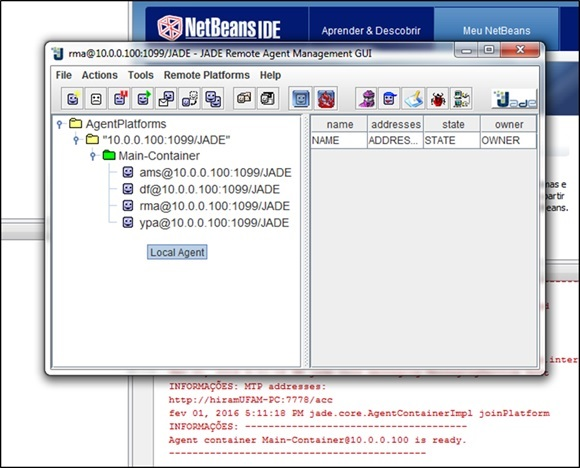
\includegraphics[width=10cm, height=6cm]{F109_SIAPE_YPA.jpg} 
					\caption{Plataforma Jade - Agente YPA}
					\label{F109}
				\end{figure}
			
			
	\textbf{5.} Criar um agente AcHw -
			Ainda dentro da plataforma Jade, criar um container, e dentro dele criar um agente AcHw. O agente Acesso Hardware é o responsável por fornecer os módulos presentes na interface elétrica ao YPA; 
			
				\begin{figure}[!h]
					\centering
					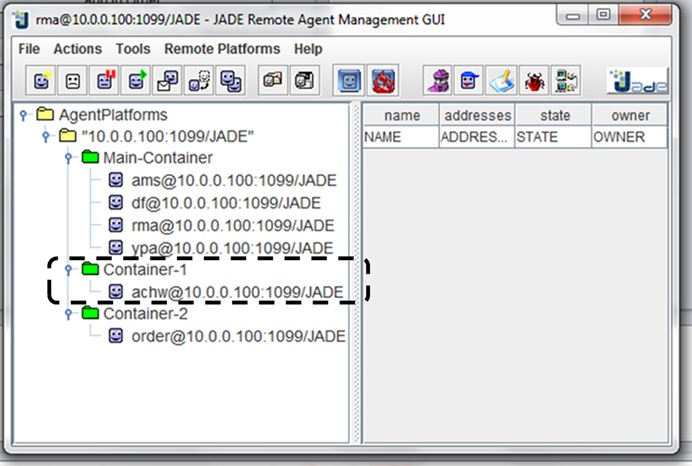
\includegraphics[width=10cm, height=5cm]{F110_SIAPE_AcHw.jpg} 
					\caption{Plataforma Jade -- Agente AcHw}
					\label{F110}
				\end{figure}
			
		\textbf{6.} Criar um agente Order.
			Criar um segundo container, e dentro desse criar um agente Order. O agente Order é o agente que instancia a interface anagrama responsável em receber as informações do cliente, e depois que receber o plano do agente Order, realizar esse plano.
%		\end{description}
			
				\begin{figure}[!h]
					\centering
					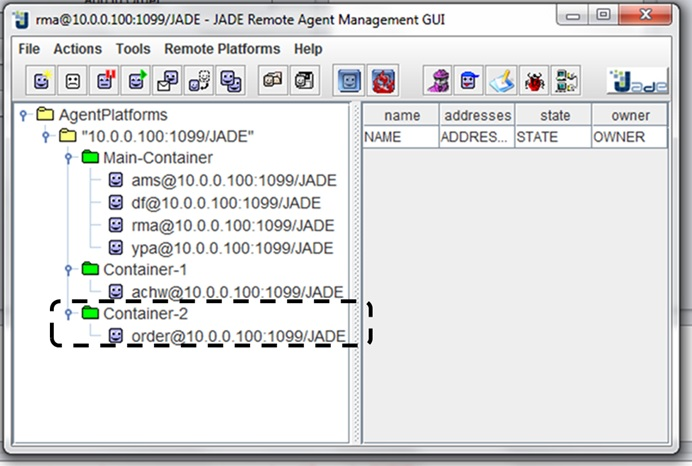
\includegraphics[width=10cm, height=5cm]{F111_SIAPE_ORDER.jpg} 
					\caption{Plataforma Jade - Agente Order}
					\label{F111}
				\end{figure}
		
		Quando o agente Order é criado, ele instancia o agente Anagrama que fica acessível ao operador por meio da interface gráfica. O operador deverá inserir os pedidos do cliente na interface, essa atividade inicia o estudo de caso propriamente dito, e este é descrito na próxima seção deste capítulo.
		
	\newpage
	
		
\section{Realização da experimentação}


Nesta seção o estudo de caso é realizado, isto é, a solicitação do cliente é inserida no sistema pelo operador, o sistema realiza a produção e retorna ao operador os pedidos do cliente na forma de produtos. Esses produtos são entregues ao cliente, atividade que conclui o estudo de caso. Além da realização, os resultados são registrados para que possam ser analisados na próxima seção. \par 

Da mesma forma que foi feito na seção anterior, os procedimentos de 7 a 11 serão realizados e podem ser acompanhados com as ilustrações de cada atividade e pela ilustração da Figura \ref{F105}.
		
		\textbf{7.} O operador insere os pedidos do clientes na Interface gráfica Anagrama.

	O operador segue os procedimento para inserir anagramas na interface gráfica, conforme ilustrado na Figura \ref{F142}. Na ilustração pode-se evidenciar dois pedidos do cliente inseridos na interface gráfica. Note-se que a letra E não está presente no sistema e a palavra UEA não foi inserida no plano de produção. Isso se deve ao fato do sistema não permitir que um recurso inexistente no processo seja utilizado no plano, evitando assim erro do operador.
	\begin{description}
		\item[Pedido 1 -] Produto: A  palavra UFAM; Quantidade = 03 unidades
		\item[Pedido 2 -] Produto: B  palavra UTAM; Quantidade = 04 unidades
	\end{description} 
		
			\begin{figure}[!h]
				\centering
				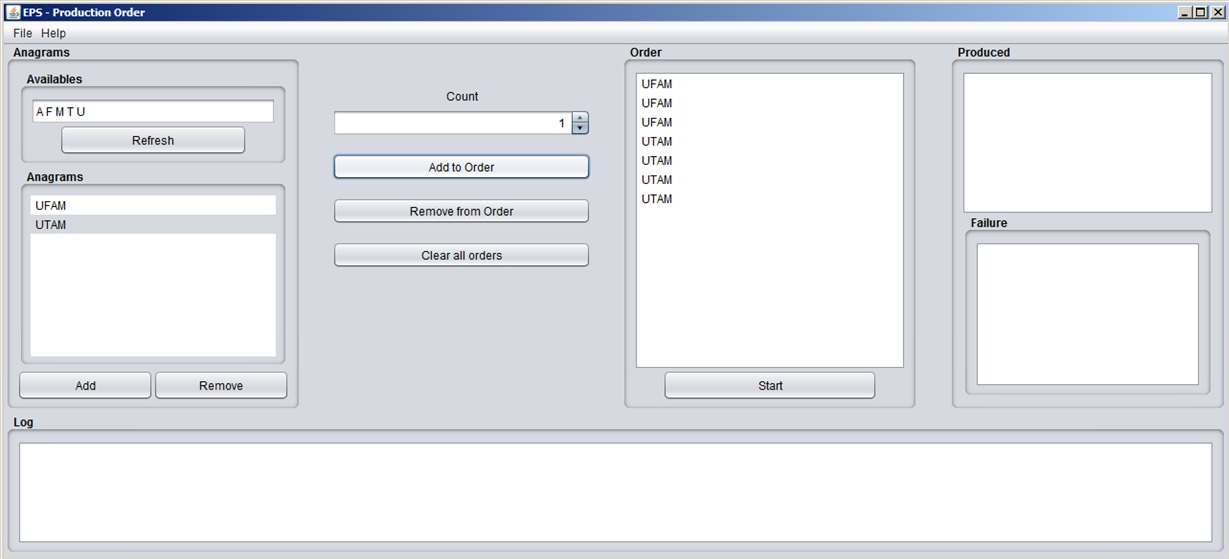
\includegraphics[width=16cm, height=9.5cm]{F142_PLANO1.jpg} 
				\caption{Plano de produção montado}
				\label{F142}
			\end{figure}
		
		
			\textbf{8.} - O operador inicia o plano de produção.

No momento em que o operador inicia o plano de produção, o agente Anagram extende do agente Produto as informações para a realização de um produto, neste caso, a palavra UFAM. A Figura\ref{F147} ilustra um trecho do código. 

	
	\begin{figure}[!h]
		\centering
		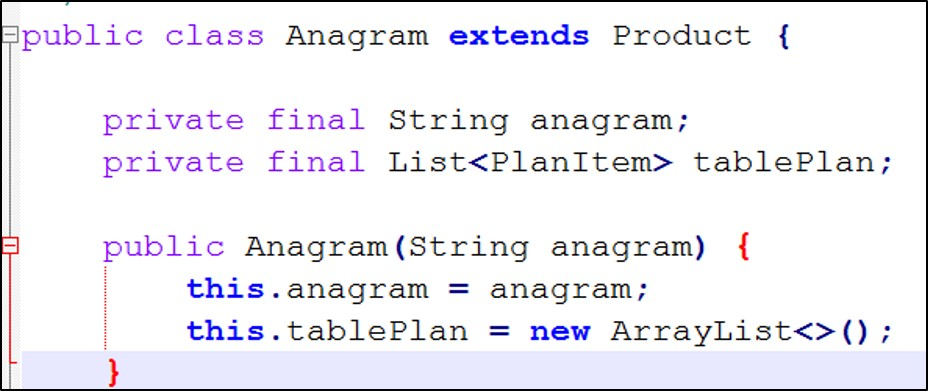
\includegraphics[width=11cm, height=4.5cm]{F147_extends.jpg} 
		\caption{SIAPE: trecho extends}
		\label{F147}
	\end{figure}
	
	Neste momento o agente Produto instancia o agente Anagram com os parâmetros necessários à produção da palavra UFAM e o seguinte método é realizado:
	
	1) É definido o agente AcHw com os parâmetros que deverão ser configurados para realizar a produção conforme ilustrado na Figura \ref{F148}:

		\begin{figure}[!h]
			\centering
			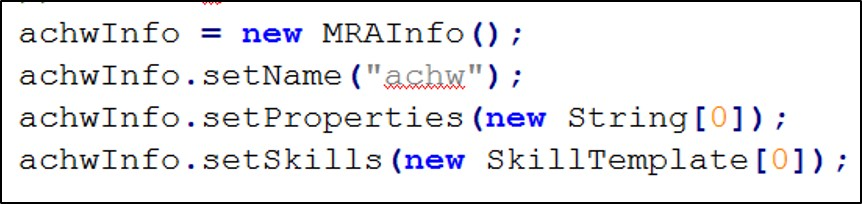
\includegraphics[width=10cm, height=2.5cm]{F148_achw.jpg} 
			\caption{SIAPE: trecho achw}
			\label{F148}
		\end{figure}
	
	2) As letras disponíveis no sistemas ficam acessíveis para ser utilizadas no processo de montagem de acordo com as solicitações do operador. A Figura \ref{F149} ilustra o trecho desse código.
	
		\begin{figure}[!h]
			\centering
			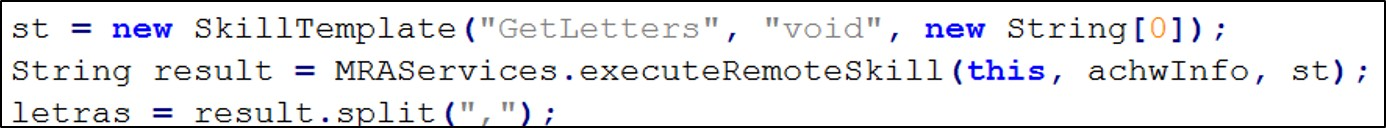
\includegraphics[width=14cm, height=1.8cm]{F149_letters.jpg} 
			\caption{SIAPE: trecho GetLetters}
			\label{F149}
		\end{figure}
	
	3) A Figura \ref{F150} ilustra o plano de produção que é criado utilizando-se as letras disponíveis que são organizadas conforme a sequência, primeiramente, da posição do módulo e depois, da posição da letra no palete.
	
		\begin{figure}[!h]
			\centering
			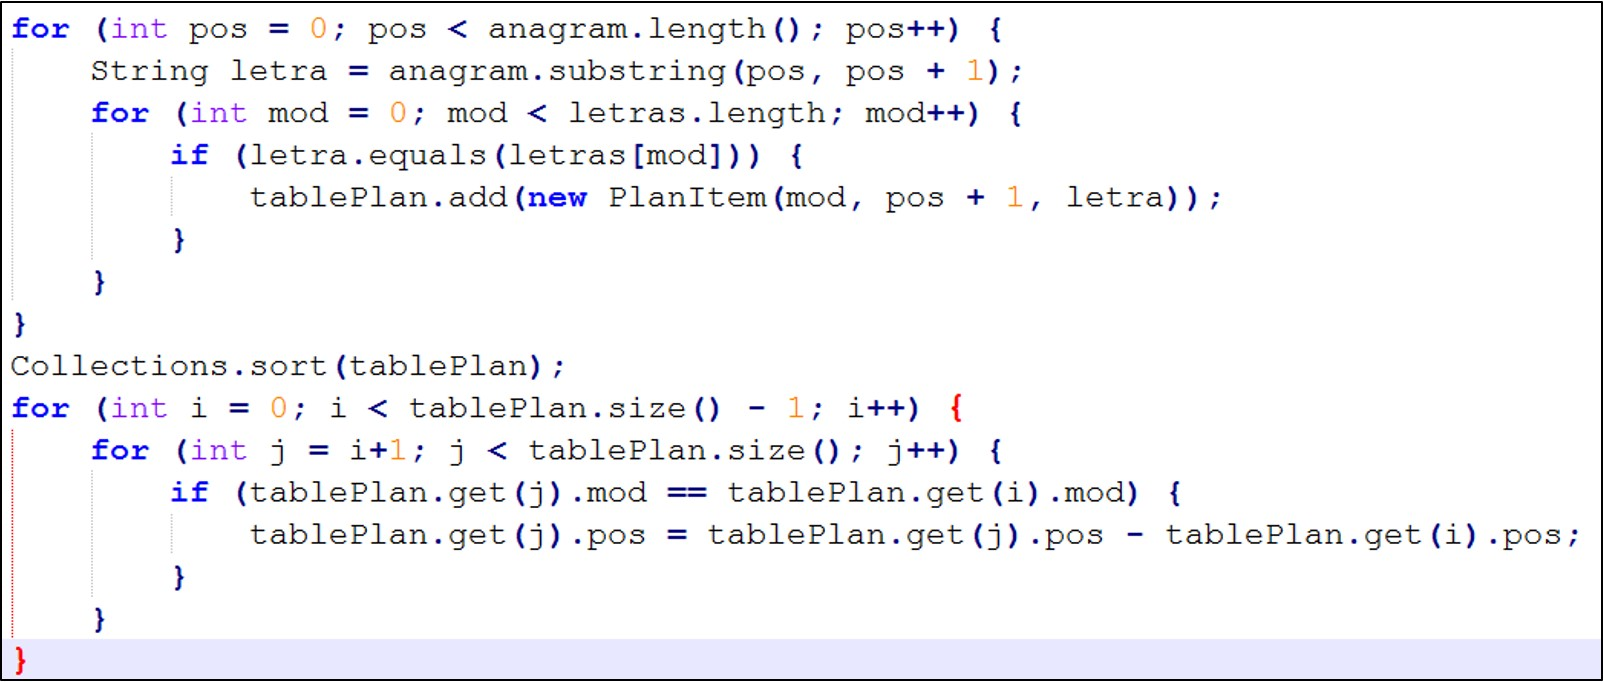
\includegraphics[width=16cm, height=7cm]{F150_criaPlano.jpg} 
			\caption{SIAPE: trecho tablePlan}
			\label{F150}
		\end{figure}
	
	4) Uma vez que as letras são organizada o plano é executado por meio dos skills MoveToStart do agente AcHw. Esse trecho do código está ilustrado na Figura \ref{F151}:
	
		\begin{figure}[!h]
			\centering
			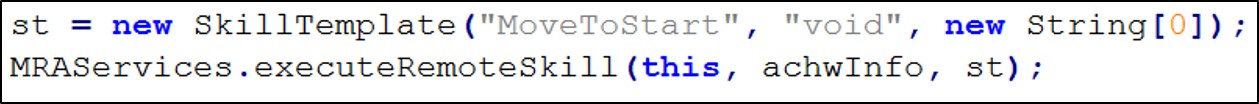
\includegraphics[width=15cm, height=1cm]{F151_MoveTo.jpg} 
			\caption{SIAPE: trecho MoveToStart}
			\label{F151}
		\end{figure}
	5)O palete é movido até o módulo do sistema especificado para a posição definida no palete. Esse método é repetido até que a produção da palavra definida seja concluída, no caso do exemplo do experimento, a palavra UFAM. A Figura \ref{F152} ilustra o trecho do código.

		\begin{figure}[!h]
			\centering
			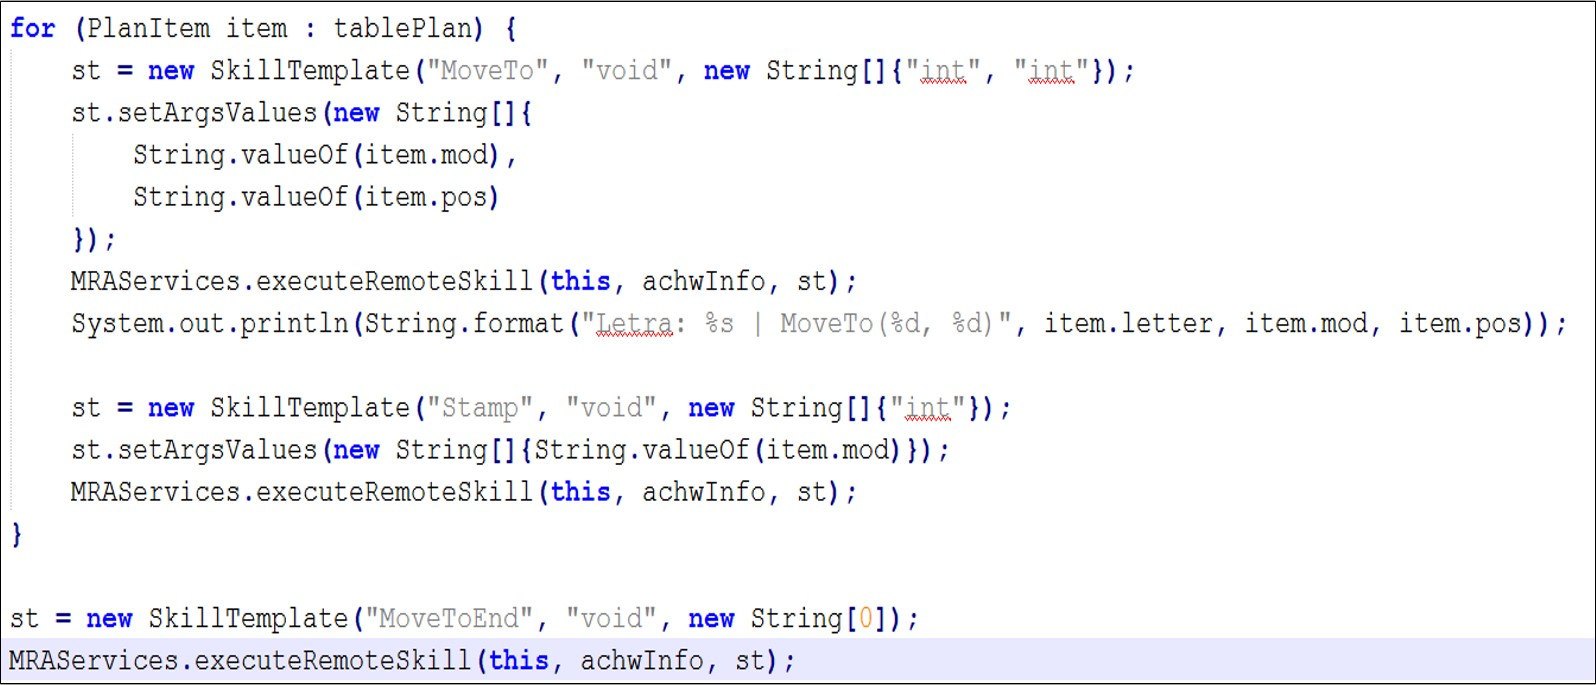
\includegraphics[width=16cm, height=7cm]{F152_MoveToEnd.jpg} 
			\caption{SIAPE: trecho MoveToEnd}
			\label{F152}
		\end{figure}
	
	6) Após realização da produção a situação da produção é informada na tela -- conforme Figura \ref{F153} -- o resultado é mostrado no tela:
			
			\begin{figure}[!h]
				\centering
				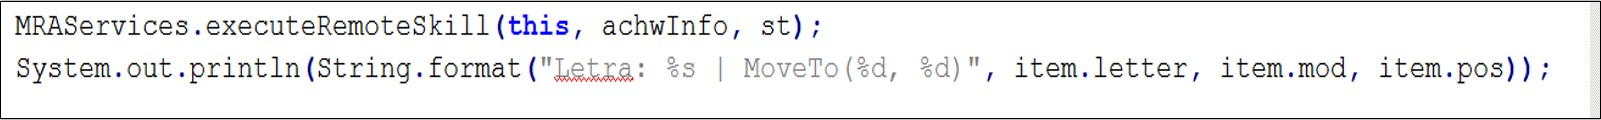
\includegraphics[width=15cm, height=2cm]{F153_PrintStatus.jpg} 
				\caption{SIAPE: trecho Status}
				\label{F153}
			\end{figure}
	
	A Figura \ref{F146} mostra um instantâneo da finalização da produção da palavra UFAM e início da palavra UTAM. Note-se que a diferença entre as duas palavras é a letra que se encontra na segunda posição do palete, ou seja, para a letra F, têm-se o seguinte skill MoveTo(1,2), indicando a atuação do módulo 1 (letra F) na posição 2 do palete. Para a letra T, têm-se o seguinte skill MoveTo(3,2), indicando a atuação do módulo 3 (letra T) na posição 2 do palete.

	\begin{figure}[!h]
		\centering
		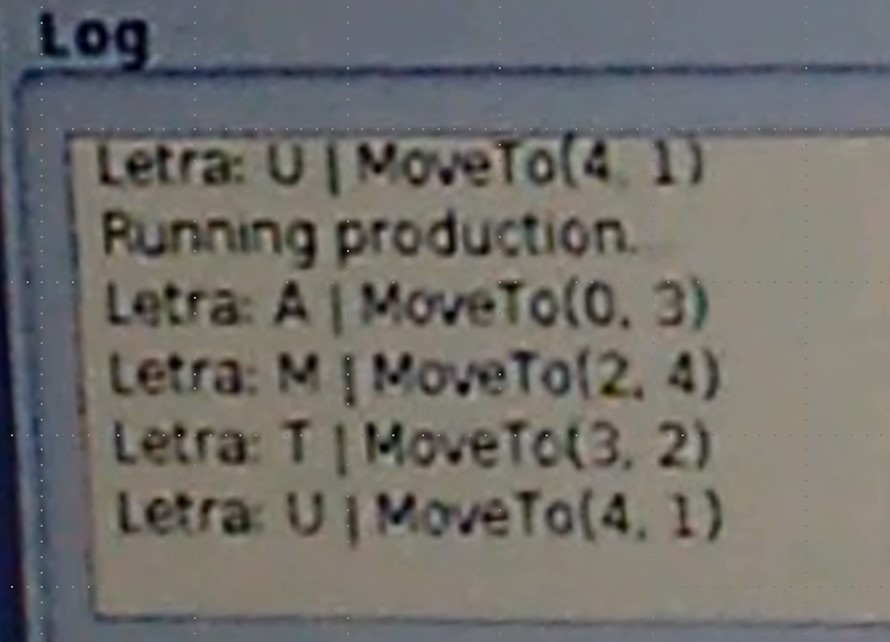
\includegraphics[width=9cm, height=4cm]{F146_LOG.jpg} 
		\caption{Log passagem UFAM para UTAM}
		\label{F146}
	\end{figure}


	Do ponto de vista do operador quando a tecla \textit{start} é pressionada o plano começa a ser produzido obedecendo a sequência definida no plano de produção. Na Figura \ref{F113} pode ser evidenciado que os dois primeiros lotes de produção, relativos aos pedidos A e B já foram produzidos e o terceiro lote será o próximo a ser produzido. Note-se que os produtos A e B usam recursos diferentes (letras T e F) e, nem por isso, houve a necessidade de se parar o sistema para que o recurso fosse trocado de posição. Importante também notar que as quantidades dos produtos também são diferentes (A=3 e B=4) e não houve qualquer parada para a alteração da quantidade, isto é, tanto o tipo de recurso quanto a quantidade dos lotes foram alterados em tempo real durante a produção dos produtos A e B.\par 
	O instantâneo mostrado na Figura \ref{F113} também registrou a presença do recurso E (letra E). Isso se deve ao procedimento do operador trocar o módulo da letra T pelo módulo da letra E e atualizar o sistema sem ter que desligar  sistema. Uma vez atualizado, o módulo foi imediatamente incluído no plano de produção e realizado no processo de produção.  
	
		\begin{description}
			\item[Pedido 3 -] Produto: C  palavra UEA; Quantidade = 05 unidades
		\end{description} 
	
		\begin{figure}[!h]
			\centering
			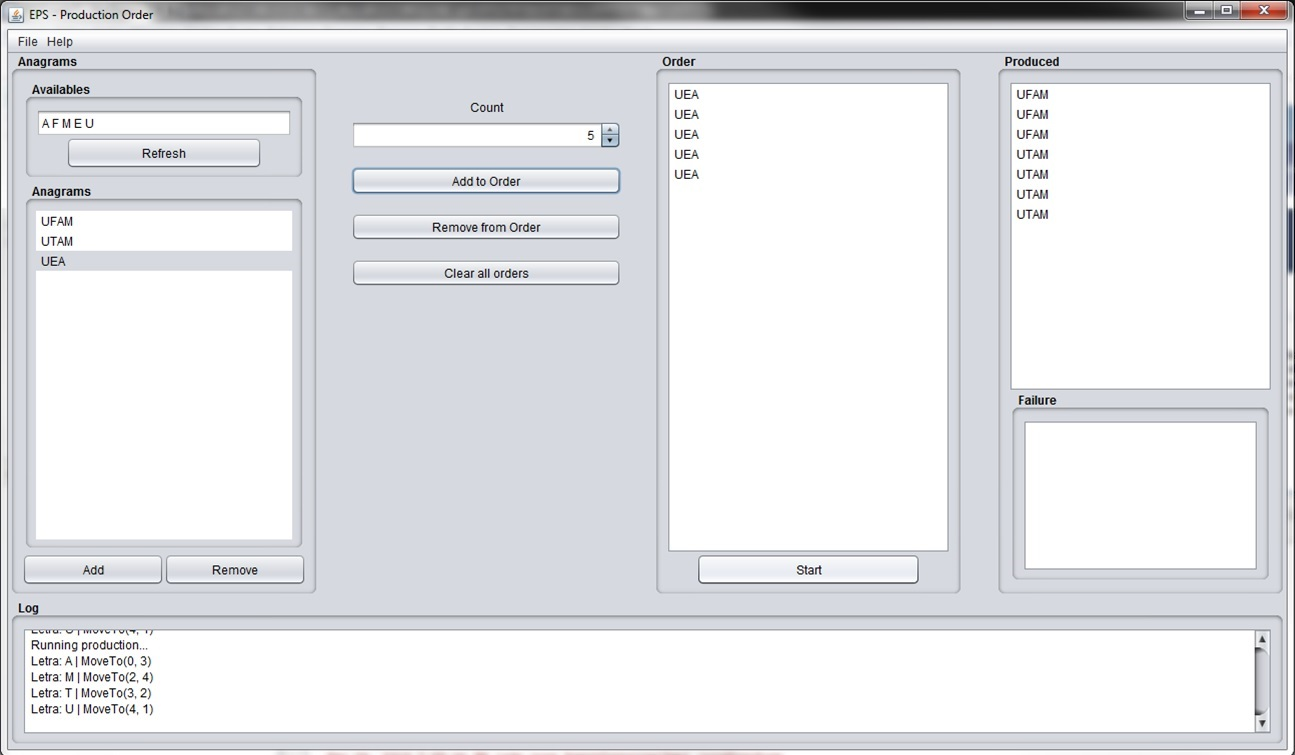
\includegraphics[width=16cm, height=8cm]{F113_SIAPE_PLANO_2_3.jpg} 
			\caption{Realizando Plano de produção}
			\label{F113}
		\end{figure}
		
		Um olhar mais atento às Figuras \ref{F142} e \ref{F113} e às operações realizadas, percebe-se a realização do conceito \textit{plug and produce} pois o tempo necessário para realizar a troca de módulos entre os produtos B e C, a atualização e a inserção do produto C no plano de produção foi em média de 42,25 segundos, que na prática, esta operação representa a troca de um produto com o sistema em funcionamento sendo praticamente nula comparada aos tempos praticados hoje em dia que ficam em torno de 30 a 45 minutos, dependendo do número de recursos que compõem  produto. É claro que há de se considerar o nível reduzido da experimentação realizada, contudo, como as operações realizadas foram possibilitadas devido às características do sistema que são dinâmicas, esses ganhos tendem a se repetir em plantas reais, pois a dinâmica que reconhece e atualiza o sistema se dá no nível de software.\par 
		Outro detalhe importante a ser notado é que o sistema não permite que um recurso (letra) seja inserido no plano sem que o mesmo esteja presente no sistema. Caso ocorra uma falha, como, por exemplo, a retirada de um módulo durante o processo produtivo, o erro é identificado e o sistema não permite que o produto seja produzido. Para que o sistema continue, o recurso pode ser reinserido para que a produção do produto continue.\par    
		
		
		\textbf{9.} O operador recebe a confirmação da realização do plano. Por meio da Figura \ref{F114} pode-se evidenciar que o plano foi totalmente realizado sem nenhuma falha. Note-se que o campo failure está vazio, indicando que que a performance do sistema nesse plano foi 100\%.
		
		
			\begin{figure}[!h]
				\centering
				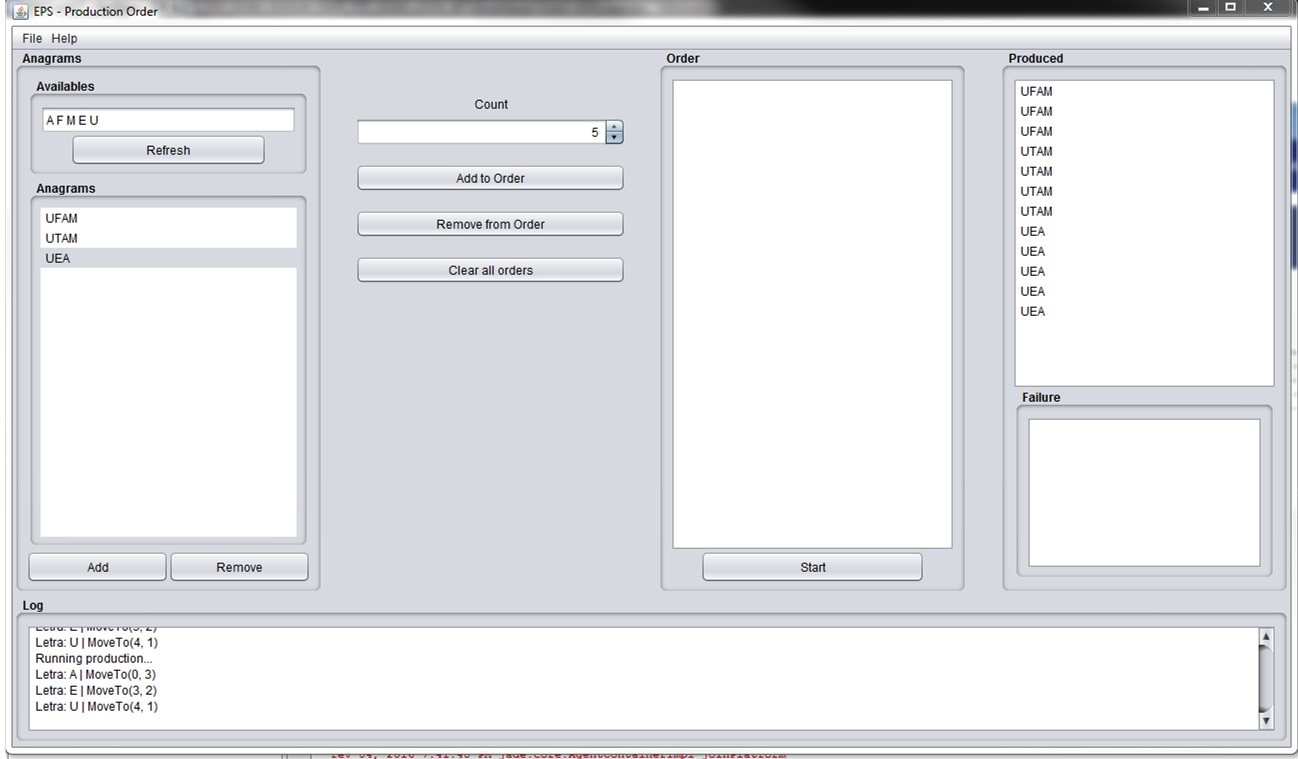
\includegraphics[width=16cm, height=8cm]{F114_SIAPE_PLANO_3_3.jpg} 
				\caption{Interface gráfica com Plano de produção}
				\label{F114}
			\end{figure}
		
		
		\textbf{10.} O operador entrega os produtos e desliga o sistema. 
		
		
		Após a confirmação da realização da experimentação de produção no SIAPE, o operador desliga o sistema e separa os lotes para serem entregues conforme os pedidos dos produtos e suas respectivas quantidades. Entregues os lotes a experimentação está concluída.
		
		A próxima seção analisa os resultados registrados nesta seção e discute os processamentos realizados pelos agentes do sistema.
		
		\begin{center}
		
		\end{center}	
			
		A realização da experimentação evidenciou de uma forma simplificada e operacional a funcionalidade do  SIAPE, isto é, as funcionalidade que interessam especificamente ao cliente, pois com o sistema, as necessidades do cliente tendem a ser atendidas e os seus problemas solucionados.\par 
		Além de evidenciar as funcionalidades do sistema, foi possível utilizar o manual de instruções e realizar os passos necessários para realizar os pedidos solicitados, neste casos, o plano de produção contendo os produtos ilustrados na Figura  \ref{F115}. Nos detalhes, visão dos lotes e a  finalização de um produto.\par
		
		\begin{figure}[!h]
			\centering
			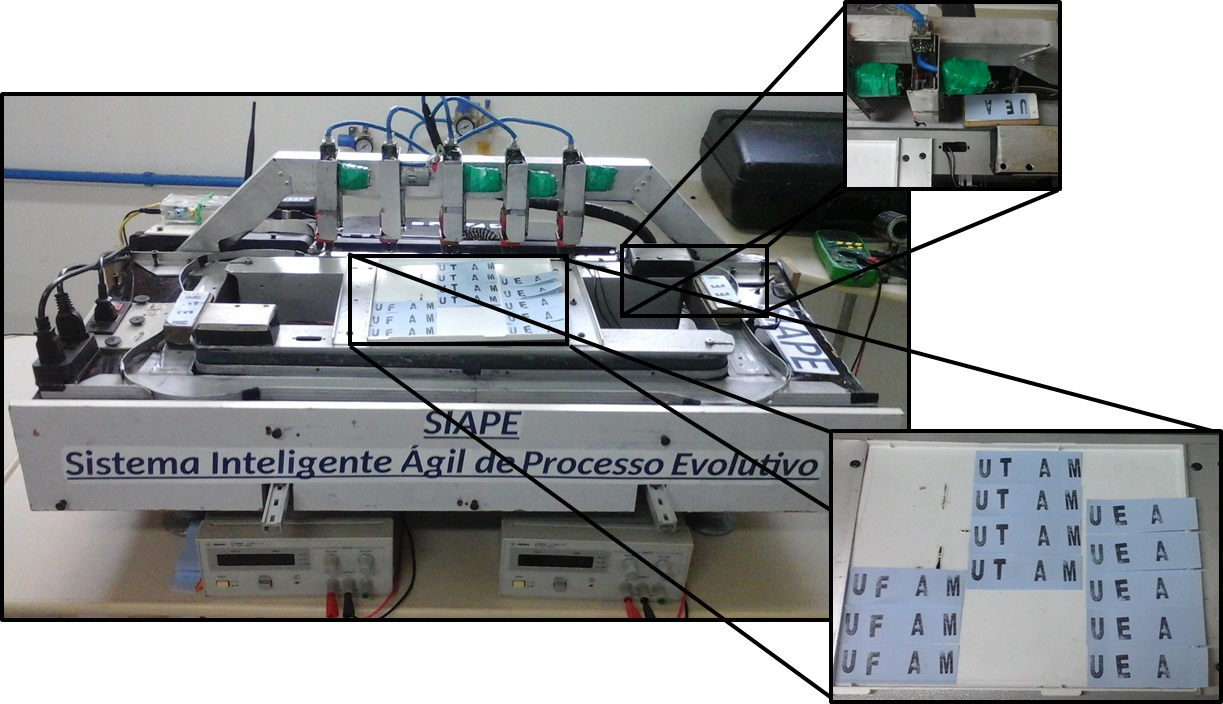
\includegraphics[width=16cm, height=8cm]{F115_SIAPE_Finalizacao_do_Plano_de_Producao.jpg} 
			\caption{Plano de produção realizado}
			\label{F115}
		\end{figure}
		
		Ao final da experimentação o sistema foi ligado, configurado, operado para realizar os produtos. O resultado da produção foi finalmente,   entregue ao cliente. Contudo, existem outras questões que devem ser melhor detalhadas e discutidas como por exemplo:\par 
		1. Como se comportaram os valores temporais e a performance do sistema? \par 
		2. A questão do paradigma evolutivo como potencial solução da customização de massa, ficou evidenciada com a experimentação?\par 
		3. Como ficou a relação entre os referenciais internos e externos e suas  implicações sobre a ciência, a tecnologia e a inovação? \par 
		Essas questões são abordadas no Capítulo 5, a seguir, que analisa os resultados da pesquisa. 
		
		%O sistema foi ligado, configurado, operado para realizar os produtos. O resultado da produção foi finalmente,   entregue ao cliente. Contudo, existem outras questões em níveis mais elevados que devem ser discutidas de uma forma mais detalhada, por exemplo, como se comportaram os valores temporais e a performance do sistema? A questão do paradigma evolutivo como potencial solução da customização de massa, ficou evidenciada com a experimentação? Como ficou a relação entre os referencias internos e externos e suas  implicações sobre a ciência, a tecnologia e a inovação. Essas questões são abordadas no Capítulo 5 que analisa os resultados da pesquisa. 
	